\chapter{Sistemi Numerici}
\section{Introduzione}
L'aritmetica svolta dai computer differice dall'aritmetica a noi familiare, i motivi sono molteplici, ma quello prinicipale è sicuramente da attribuire alla diversa modalità neòòa rappresentazione dei dati e delle informazioni.

\begin{align*}
    16_{10} & \neq 16_{16} \quad \text{(16 in decimale è diverso da 16 in esadecimale)} \\[8pt]
    16_{10} &= 1 \cdot 10^1 + 6 \cdot 10^0 = 16_{10} \\
    16_{16} &= 1 \cdot 16^1 + 6 \cdot 16^0 = 22_{10}
\end{align*}

Se per noi il sistema decimale può sembrare scontato, non è certo lo stesso per i computer, infatti, i calcolatori lavorano sfruttando il sistema binario.

\section{Bit}
\subsection{Definizione}
Con il termine \textbf{bit} definiamo l'unità di misura dell'informazione, un bit \uline{può assumere solo il valore di 0 o 1}

\subsection{Unità di misura}
Combinando tra loro più bit si ottengono strutture complesse, in particolare:
\begin{itemize}
    \item Byte - 8 bit
    \item Nybble - 4 bit
    \item Word - 32 bit
    \item Halfword - 16 bit
    \item Doubleword - 64 bit
\end{itemize}

\subsection{Numero di configurazione possibili}
Dati \textbf{k bit} il \uline{numero di configurazione ottenibili è pari a $2^k$}

\newpage
\section{Rappresentazione di un sistema numerico posizionale}
\subsection{Cosa è un sistema numerico posizionale?}
È un sistema numerico dove ogni cifra assume un valore diverso a seconda della posizione che occupa all'interno del numero

\subsection{Formula}
\begin{tcolorbox}
    {
        \LARGE
        $$
            N = \sum^{n-1}_{i=-m} d_i \cdot r^i
        $$
    }
    \begin{itemize}
        \item[$d$ -] rappresenta la singola cifra
        \item [$r$ -] è la radice o base del sistema
        \item [$n$ -] è il numero di cifre della parte intera (sinistra della virgola)
        \item [$m$ -] è il numero di cifre della parte frazionaria (destra della virgola)
    \end{itemize}
    
    \subsubsection{Esempio d'uso formula}
    {
        \Large
        \begin{gather*}
            15 = 10 \cdot 10^1 + 5 \cdot 10^0
        \end{gather*}
    }
\end{tcolorbox}

\section{Sistema Binario}
\subsection{Definizione}
\begin{itemize}
    \item Base: $r=2$
    \item Cifre: $d=0,1$
    \item Un valore numerico $N$ si rappresenta come:
    {\large
        $$
            N = d_{n-1} \cdot 2^{n-1} + \dots + d_0 \cdot 2^0 + d_{-1} \cdot 2^{-1} + \dots + d_{-m} \cdot 2^{-m}
        $$
    }
\end{itemize}

\subsection{Esempio}
{
    \Large
    $$
        101_2 = 1 \cdot 2^2 + 0 \cdot 2^1 + 1 \cdot 2^0 = 5_{10}
    $$
}

\subsection{Byte}
È una sequenza di otto bit consecutivi

\begin{center}
    \begin{minipage}{0.3\textwidth}
        \begin{center}
            
            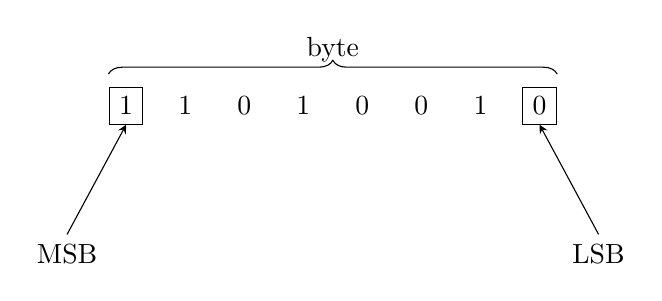
\begin{tikzpicture}[x=0.5cm, y=0.5cm, >=stealth, scale=1.5]
            
                % 1. BIT INDIVIDUALI (Garantisce allineamento perfetto)
                \node (b7) at (0,0) {1};
                \node (b6) at (1,0) {1};
                \node (b5) at (2,0) {0};
                \node (b4) at (3,0) {1};
                \node (b3) at (4,0) {0};
                \node (b2) at (5,0) {0};
                \node (b1) at (6,0) {1};
                \node (b0) at (7,0) {0};
            
                % 2. REPTANGOLI SU MSB (b7) E LSB (b0)
                \draw (b7.south west) rectangle (b7.north east);
                \draw (b0.south west) rectangle (b0.north east);
            
                % 3. GRAFFA SUPERIORE
                \draw[decorate, decoration={brace, amplitude=5pt, raise=3pt}] 
                    (-0.3, 0.4) -- (7.3, 0.4) 
                    node[midway, yshift=12pt] {byte};
            
                % 4. TESTI MSB / LSB
                \node (msb) at (-1, -2.5) {MSB};
                \node (lsb) at (8, -2.5) {LSB};
            
                % 5. FRECCE
                \draw[->] (msb.north) -- (b7.south);
                \draw[->] (lsb.north) -- (b0.south);
            
            \end{tikzpicture}
        \end{center}
    \end{minipage}
    \hfil
    \begin{minipage}{0.33\textwidth}
        \begin{itemize}
            \item Most Significant Bit (MSB): il bit più a sinistra \\
            \item Least Significant Bit (LSB): il bit più a destra
        \end{itemize}
    \end{minipage}
\end{center}

\section{Sistema Ottale}
\subsection{Definizione}
\begin{itemize}
    \item Base $r=8$
    \item Cifre $d=0,1,\dots,7$
    \item Un valore numerico $N$ si rappresenta come:
    {\large
        $$
            N = d_{n-1} \cdot 8^{n-1} + \dots + d_0 \cdot 8^0 + d_{-1} \cdot 8^{-1} + \dots + d_{-m} \cdot 8^{-m}
        $$
    }
\end{itemize}

\subsection{Esempio}
{
    \Large
    $$
        127_8 = 1 \cdot 8^2 + 2 \cdot 8^1 + 7 \cdot 8^0 = 87_{10}
    $$
}

\section{Sistema Esadecimale}
\subsection{Definizione}
\begin{itemize}
    \item Base $r=16$
    \item Cifre $d=0,1,\dots,9, A, B, C, D, E, F$
    \item Un valore numerico $N$ si rappresenta come:
    {\large
        $$
            N = d_{n-1} \cdot 16^{n-1} + \dots + d_0 \cdot 16^0 + d_{-1} \cdot 16^{-1} + \dots + d_{-m} \cdot 16^{-m}
        $$
    }
\end{itemize}

\subsubsection{Notazione}
Spesso si usa il pendice$_{H}$ al posto del pendice$_{16}$ per indicare la base decimale oppure $0x$ davanti al numero.

Il sistema esadecimale viene spesso abbreviato come \textbf{esa} oppure \textbf{hex}

\subsection{Significato delle lettere}
{
    \LARGE
    \begin{gather*}
    A_H = 10_{10} = 1010_2 \\
    B_H = 11_{10} = 1011_2 \\
    C_H = 12_{10} = 1100_2 \\
    D_H = 13_{10} = 1101_2 \\
    E_H = 14_{10} = 1110_2 \\
    F_H = 15_{10} = 1111_2
\end{gather*}
}

\subsection{Compattezza}
Il grande vantaggio del sistema esadecimale è la compattezza dei suoi numeri, poichè la base 16 consente di utilizzare meno cifre per rappresentare un dato numero rispetto al formato binario o esadecimale
{\large
    $$
        1111\ 0101\ 1100\ 1111 \rightarrow F5CF
    $$
}

\section{Conversione tra sistemi numerici}
\subsection{Da base $r \rightarrow$ a base $10$ }
Consideriamo per il momento solo valori interi, la conversione da qualsiasi base r a base 10 avviene come segue

\begin{tcolorbox}[title ={Base r $\rightarrow$} Base 10]
    {\LARGE
        $$
        N_r = d_{n-1} \cdot r^{n-1} + \dots + d_0 \cdot r^0 = M_{10}
        $$
    }
    \begin{itemize}
        \item [$N_r$]: Il numero di partenza espresso nella base $r$
        \item [$M_{10}$]: Il numero finale ottenuto dopo la conversione, espresso in base 10
        \item [$r$]: La radice o base del sistema numerico di partenza
        \item [$n$]: Il numero totale di cifre che compongono il numero intero di partenza
        \item [$d_i$]: Le singole cifre del numero di partenza, dove $d_0$ è la cifra meno significativa e $d_{n-1}$ è quella più significativa
        \item [$i$]: La posizione di ciascuno cifra, che determina la potenza della base $r$ per cui va moltiplicata
    \end{itemize}
    \subsubsection{Esempio}
    \begin{gather*}
        1010_2 = (1 \cdot 2^3 + 0 \cdot 2^2 + 1 \cdot 2^1 + 0 \cdot 2^0)_{10} = 10_{10} \\[1ex]
        26_8 = (2 \cdot 8^1 + 6 \cdot 8^0)_{10} = 22_{10} \\[1ex]
        431_5 = (4 \cdot 5^2 + 3 \cdot 5^1 + 1 \cdot 5^0)_{10} = 116_{10}
    \end{gather*}
\end{tcolorbox}

\subsection{Da base $10 \rightarrow$ a base $r$}
Consideriamo per il momento solo valori interi

La conversione da base 10 a qualsiasi base r avviene come segure:
\begin{enumerate}
    \item Dividiamo il valore numerico N per la base r fino a quando l'ultimo quoziente è minore della base stessa(r)
    \item Prendiamo l'ultimo quoziente e tutti i resti della divisione, e procedendo dall'ultimo resto al primo, li scriviamo da sinistra verso destra
\end{enumerate}

\subsubsection{Esempi}
\begin{itemize}
    \item \textit{Esempio}: Convertire il numero 12 da base 10 a base 2
    \item $12 : 2 = 6 \text{ con resto} = 0$
    \item $6 : 2 = 3 \text{ con resto} = 0$
    \item $3 : 2 = 1 \text{ con resto} = 1$
    \item $1 : 2 = 0 \text{ con resto} = 1$
    \item quindi:
    \[
        12_{10} = 1100_2
    \]
\end{itemize}

\begin{itemize}
    \item \textit{Esempio}: convertire il numero 120 da Base 10 a Base 8
    \item $120 : 8 = 15 \text{ con resto} = 0$
    \item $15 : 8 = 1 \text{ con resto} = 7$
    \item $1 : 8 = 0 \text{ con resto } 1$
\end{itemize}
quindi:
\[
    120_{10} = 170_8
\]

\begin{itemize}
    \item \textit{Esempio}: convertire il numero 1253 da base 10 a base 16
    \item $1253 : 16 = 78 \text{ con resto} = 5$
    \item $78 : 16 = 4 \text{ con resto} = 14 = \text{E}$
    \item $4 : 16 = 0 \text{ con resto } 4$
\end{itemize}
quindi:
\[
    1253_{10} = 4\text{E}5_{16}
\]

\subsection{Da base $r \rightarrow$ a base $r'$}
Consideriamo per il momento solo valori interi

La conversione da qualsiasi base $r$ a qualsiasi base $r'$ avviene come segue:
\begin{enumerate}
    \item Convertire da base $r$ a base 10
    \item Convertire il risultato da base 10 a base $r'$
\end{enumerate}

\bigskip

\begin{center}
    \begin{tikzpicture}[
    scale= 1.5, transform shape,
    box/.style={
        draw,
        rectangle,
        very thick,
        inner sep=6pt,
        minimum height=0.8cm
    },
    -stealth % Stile per le frecce
]

    % Nodi
    \node[box] (bp) {Base $r$};
    \node[box, right=2cm of bp] (b10) {Base 10};
    \node[box, right=2cm of b10] (bq) {Base $r'$};

    % Frecce
    \draw (bp) -- (b10);
    \draw (b10) -- (bq);

    \end{tikzpicture}
\end{center}

\subsubsection{Esempi}
% --- PRIMA IMMAGINE: Da Esadecimale a Binario ---
\begin{itemize}
    \item \textit{Esempio}: Convertire il numero $\text{AB2}_{16}$ in binario.
    \item $\text{A}_{16} = 10_{10} = 1010_2$
    \item $\text{B}_{16} = 11_{10} = 1011_2$
    \item $2_{16} = 2_{10} = 0010_2$
    \item quindi
    \[
        \text{AB2}_{16} = 1010\,1011\,0010_2
    \]
\end{itemize}

\vspace{0.5cm}

% --- SECONDA IMMAGINE: Da Ottale a Binario ---
\begin{itemize}
    \item \textit{Esempio}: Convertire il numero $(516)_8$ in Binario.
    \item $5_8 = 5_{10} = 101_2$
    \item $1_8 = 1_{10} = 001_2$
    \item $6_8 = 6_{10} = 110_2$
    \item quindi
    \[
        516_8 = 101001110_2
    \]
\end{itemize}

\vspace{0.5cm}

\begin{itemize}
    \item E se dovessimo convertire un numero da base 2 a base 8?
    \[
        101011_2 = ???????_8
    \]
    Svolgimento: raggruppiamo i bit a 3 a 3 da destra: $(101)_2$ e $(011)_2$
    \begin{itemize}
        \item $101_2 = 5_8$
        \item $011_2 = 3_8$
    \end{itemize}
    quindi:
    \[
        101011_2 = 53_8
    \]

    \vspace{0.3cm}

    \item Oppure da base 8 a base 2?
    \[
        5371_8 = ????_2
    \]
    Svolgimento: convertiamo ogni cifra ottale in un gruppo di 3 bit:
    \begin{itemize}
        \item $5_8 = 101_2$
        \item $3_8 = 011_2$
        \item $7_8 = 111_2$
        \item $1_8 = 001_2$
    \end{itemize}
    quindi:
    \[
        5371_8 = 101011111001_2
    \]

    \vspace{0.3cm}

    \item E da base 8 a base 16?
    \[
        742_8 = ????_{16}
    \]
    Svolgimento: 
    \begin{enumerate}
        \item Passiamo prima in binario (3 bit per cifra ottale):
        \[
            742_8 = \underbrace{111}_{7}\,\underbrace{100}_{4}\,\underbrace{010}_{2\,(2)} = 111100010_2
        \]
        \item Convertiamo da binario a esadecimale raggruppando a 4 bit da destra:
        \[
            (0001)(1110)(0010)_2
        \]
        \begin{itemize}
            \item $0001_2 = 1_{16}$
            \item $1110_2 = 14_{10} = \text{E}_{16}$
            \item $0010_2 = 2_{16}$
        \end{itemize}
    \end{enumerate}
    quindi:
    \[
        742_8 = 1\text{E}2_{16}
    \]
\end{itemize}

\newpage
\section{Rappresentazioni dei valori}
\subsection{Limite di cifre}
La rappresentazione dei valori è legata al numero di cifre disponibili, nei sistemi di elaborazione, come in generale in tutte le applicazioni pratiche,\uline{ il numero di cifre impiegate nella rappresentazioni di valori numerici è limitato.}

Si ha \textbf{overflow} quando si è nell'\uline{impossibilità di rappresentare il risultato di una operazione con il numero di cifre a disposizione}

\subsection{Tabella numeri rappresentabili}
\begin{table}[h!]
\centering
\begin{tabular}{|c|c|c|}
\hline
\begin{tabular}[c]{@{}c@{}}\textit{n}\\ numero\\ di bit\end{tabular} & 
\begin{tabular}[c]{@{}c@{}}$2^n$\\ numero di\\ valori\end{tabular} & 
\begin{tabular}[c]{@{}c@{}}$2^n-1$\\ max valore\\ rappresentabile\end{tabular} \\ \hline
1 & 2  & 1  \\ 
2 & 4  & 3  \\ 
3 & 8  & 7  \\ 
4 & 16 & 15 \\ 
5 & 32 & 31 \\ 
6 & 64 & 63 \\ 
\dots & \dots & \dots \\ \hline
\end{tabular}
\end{table}

\subsection{Prefissi}
{
    \LARGE

    \begin{gather*}
    \text{Kilo} = 2^{10} = 1024 \\
    \text{Mega} = 2^{20} = 1048576 \\
    \text{Giga} = 2^{30} = 1073741824
\end{gather*}}